\documentclass[12pt,a4paper]{article}

% ====== ENCODING & FONT ======
\usepackage[utf8]{inputenc}    % Hỗ trợ UTF-8
\usepackage[T5]{fontenc}       % Font encoding cho tiếng Việt
\usepackage[vietnamese]{babel} % Ngôn ngữ tiếng Việt

% ====== GEOMETRY & LAYOUT ======
\usepackage{geometry}          % Tùy chỉnh lề
\geometry{
  a4paper,
  top=25mm,
  bottom=25mm,
  left=25mm,
  right=25mm
}

\usepackage{setspace}          % Chỉnh khoảng cách dòng
\onehalfspacing                % Giãn dòng 1.5

\usepackage{parskip}           % Tự động thêm khoảng cách giữa các đoạn
\setlength{\parindent}{0pt}    % Không thụt đầu dòng

% ====== MATHEMATICS ======
\usepackage{amsmath, amssymb, amsfonts} % Toán học nâng cao
\usepackage{mathtools}                  % Bổ sung cho amsmath

% ====== GRAPHICS & FIGURES ======
\usepackage{graphicx}          % Thêm hình ảnh
\usepackage{float}             % Quản lý vị trí hình/table
\usepackage{caption}           % Tùy chỉnh caption
\usepackage{subcaption}        % Sub-figures

% ====== TABLES ======
\usepackage{array}             % Cải tiến bảng
\usepackage{booktabs}          % Dòng bảng đẹp hơn
\usepackage{multirow}          % Gộp ô bảng theo chiều dọc
\usepackage{multicol}          % Gộp cột
\usepackage{longtable}         % Bảng dài nhiều trang
\usepackage{tabularx}          % Bảng có chiều rộng tự động

% ====== COLORS & HYPERLINKS ======
\usepackage[dvipsnames]{xcolor} % Màu sắc mở rộng
\usepackage{hyperref}           % Tạo liên kết
\hypersetup{
    colorlinks=true,
    linkcolor=blue,
    urlcolor=blue,
    citecolor=blue,
    pdfborder={0 0 0}
}

% ====== LISTS ======
\usepackage{enumitem}           % Tùy chỉnh danh sách
\setlist[itemize]{noitemsep}    % Giảm khoảng cách itemize
\setlist[enumerate]{noitemsep}

% ====== HEADER & FOOTER ======
\usepackage{fancyhdr}
\pagestyle{fancy}
\fancyhf{}
\fancyhead[L]{\leftmark}  % Tiêu đề bên trái
\fancyhead[R]{\thepage}   % Trang bên phải

% ====== OTHER UTILITIES ======
\usepackage{pdfpages}          % Chèn file PDF
\usepackage{lipsum}            % Sinh text giả (demo)
\usepackage{titlesec}          % Tùy chỉnh tiêu đề
\titleformat{\section}{\large\bfseries}{\thesection}{1em}{}
\titleformat{\subsection}{\normalsize\bfseries}{\thesubsection}{1em}{}


\begin{document}

\textbf{PHẦN I. Câu trắc nghiệm nhiều phương án lựa chọn.} Thí sinh trả
lời từ câu 1 đến câu 12. Mỗi câu thí sinh chỉ chọn một phương án.

\begin{enumerate}
\def\labelenumi{\arabic{enumi}.}
\item
  Cho hàm số \(y = f(x)\) có bảng biến thiên như sau:
\end{enumerate}

\begin{quote}
\begin{center}

\includegraphics[width=4.29792in,height=1.28056in]{./media/image1.png}
\end{center}

Giá trị cực đại của hàm số đã cho bằng

\textbf{A.} \(3\). \textbf{B.} \(- 1\). \textbf{C.} \(- 5\). \textbf{D.}
\(1\).
\end{quote}

\begin{enumerate}
\def\labelenumi{\arabic{enumi}.}
\setcounter{enumi}{1}
\item
  Cho hàm số \(y = f(x)\) liên tục và có bảng biến thiên trên đoạn
  \(\lbrack - 1;3\rbrack\) như hình vẽ bên. Khẳng định nào sau đây
  \emph{\textbf{đúng}}?
\end{enumerate}

\begin{quote}
\begin{center}
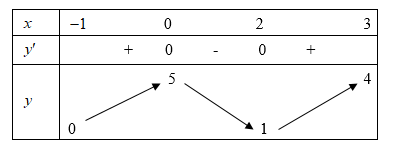
\includegraphics[width=3.64583in,height=1.38889in]{./media/image2.png}
\end{center}

\textbf{A.} \(\max_{\lbrack - 1;3\rbrack}f(x) = f(0)\).
\textbf{B.}\(\max_{\lbrack - 1;3\rbrack}f(x) = f(3)\).

\textbf{C.} \(\max_{\lbrack - 1;3\rbrack}f(x) = f(2)\). \textbf{D.}
\(\max_{\lbrack - 1;3\rbrack}f(x) = f( - 1)\).
\end{quote}

\begin{enumerate}
\def\labelenumi{\arabic{enumi}.}
\setcounter{enumi}{2}
\item
  Cho hàm số \(y = f(x)\) có đồ thị như hình vẽ.
\end{enumerate}

\begin{quote}
\begin{center}
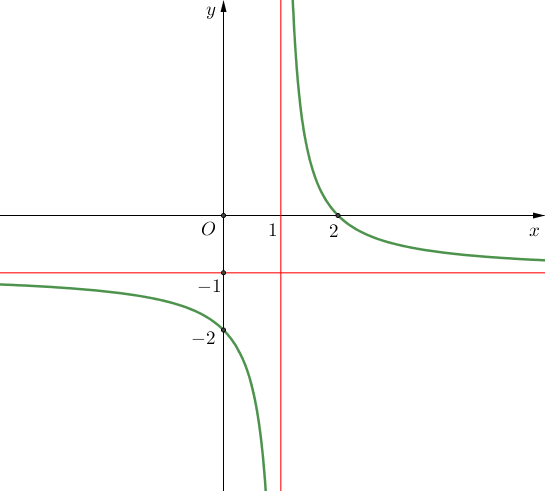
\includegraphics[width=3.07639in,height=2.68056in]{./media/image3.png}
\end{center}

Đồ thị hàm số đã cho có đường tiệm cận đứng bằng:

\textbf{A.} \(x = 1\). \textbf{B.} \(x = - 1\). \textbf{C.} \(x = 0\).
\textbf{D.}\(y = - 1\)
\end{quote}

\begin{enumerate}
\def\labelenumi{\arabic{enumi}.}
\setcounter{enumi}{3}
\item
  Tìm đường tiệm cận xiên của đồ thị hàm số
  \(f(x) = \frac{x^{2} + 3x}{x - 2}\).
\end{enumerate}

\begin{quote}
\textbf{A.} \(y = 2x - 5\). \textbf{B.} \(y = x - 2\). \textbf{C.}
\(y = x + 5\). \textbf{D.} \(y = x - 5\).
\end{quote}

\begin{enumerate}
\def\labelenumi{\arabic{enumi}.}
\setcounter{enumi}{4}
\item
  Đường cong hình bên là đồ thị của một trong bốn hàm số dưới đây. Hàm
  số đó là hàm số nào?
\end{enumerate}

\begin{quote}
\begin{center}
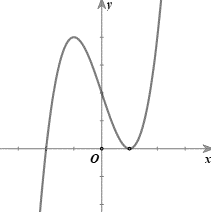
\includegraphics[width=2.18056in,height=1.84028in]{./media/image4.png}
\end{center}

\textbf{A.}
\(\mathbf{y =}\mathbf{-}\mathbf{x}^{\mathbf{3}}\mathbf{+ 3x + 2}\).
\textbf{B.} \(\mathbf{y =}\mathbf{x}^{\mathbf{2}}\mathbf{+ 1}\).
\textbf{C.}
\(\mathbf{y =}\mathbf{x}^{\mathbf{3}}\mathbf{+}\mathbf{x}^{\mathbf{2}}\mathbf{+ 1}\).
\textbf{D.}\(\mathbf{y =}\mathbf{x}^{\mathbf{3}}\mathbf{-}\mathbf{3x + 2}\)
\end{quote}

\begin{enumerate}
\def\labelenumi{\arabic{enumi}.}
\setcounter{enumi}{5}
\item
  Cho hình hộp \(ABCD.A'B'C'D'\). Đặt
  \(\overrightarrow{AB} = \overrightarrow{a}\),
  \(\overrightarrow{AD} = \overrightarrow{b}\),
  \(\overrightarrow{AA'} = \overrightarrow{c}\). Phân tích vectơ
  \(\overrightarrow{AC'}\) theo
  \(\overrightarrow{a},\overrightarrow{b},\overrightarrow{c}\)?
\end{enumerate}

\begin{quote}
\textbf{A.}
\(\overrightarrow{AC'} = - \overrightarrow{a} + \overrightarrow{b} + \overrightarrow{c}\).
\textbf{B.}
\(\overrightarrow{AC'} = \overrightarrow{a} + \overrightarrow{b} - \overrightarrow{c}\).
\textbf{C.}
\(\overrightarrow{AC'} = \overrightarrow{a} + \overrightarrow{b} + \overrightarrow{c}\).
\textbf{D.}
\(\overrightarrow{AC'} = \overrightarrow{a} - \overrightarrow{b} + \overrightarrow{c}\).
\end{quote}

\begin{enumerate}
\def\labelenumi{\arabic{enumi}.}
\setcounter{enumi}{6}
\item
  Trong không gian với hệ trục tọa độ \(Oxyz\), cho
  \(\overrightarrow{a} = - \overrightarrow{i} + 2\overrightarrow{j} - 3\overrightarrow{k}\).
  Tọa độ của vectơ \(\overrightarrow{a}\) là
\end{enumerate}

\begin{quote}
\textbf{A.}
\(\left( \mathbf{-}\mathbf{1;2;}\mathbf{-}\mathbf{3} \right)\).
\textbf{B.}
\(\left( \mathbf{2;}\mathbf{-}\mathbf{3;}\mathbf{-}\mathbf{1} \right)\).
\textbf{C.}
\(\left( \mathbf{2;}\mathbf{-}\mathbf{1;}\mathbf{-}\mathbf{3} \right)\).
\textbf{D.}
\(\left( \mathbf{-}\mathbf{3;2;}\mathbf{-}\mathbf{1} \right)\).
\end{quote}

\begin{enumerate}
\def\labelenumi{\arabic{enumi}.}
\setcounter{enumi}{7}
\item
  Cho tứ diện \(ABCD\). Đặt
  \(\overrightarrow{AB} = \overrightarrow{a}\),
  \(\overrightarrow{AC} = \overrightarrow{b}\),
  \(\overrightarrow{AD} = \overrightarrow{c}\). Gọi \(M\) là trung điểm
  của đoạn \(BC\). Đẳng thức nào dưới đây đúng?
\end{enumerate}

\begin{quote}
\textbf{A.}
\(\overrightarrow{DM} = \frac{1}{2}\left( \overrightarrow{a} + \overrightarrow{b} - 2\overrightarrow{c} \right)\).
\textbf{B.}
\(\overrightarrow{DM} = \frac{1}{2}\left( \overrightarrow{a} + 2\overrightarrow{b} - \overrightarrow{c} \right)\).

\textbf{C.}
\(\overrightarrow{DM} = \frac{1}{2}\left( \overrightarrow{a} - 2\overrightarrow{b} + \overrightarrow{c} \right)\).
\textbf{D.}
\(\overrightarrow{DM} = \frac{1}{2}\left( \overrightarrow{a} + 2\overrightarrow{b} - \overrightarrow{c} \right)\).
\end{quote}

\begin{enumerate}
\def\labelenumi{\arabic{enumi}.}
\setcounter{enumi}{8}
\item
  Giá trị nhỏ nhất của hàm số
  \begin{center}
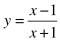
\includegraphics[width=0.625in,height=0.43403in]{./media/image5.png}
\end{center}
  trên đoạn
  \begin{center}

\includegraphics[width=0.375in,height=0.26458in]{./media/image6.png}
\end{center}
  là:
\end{enumerate}

\begin{quote}
\textbf{A.}
\begin{center}
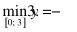
\includegraphics[width=0.80903in,height=0.33056in]{./media/image7.png}
\end{center}
\textbf{B.}
\begin{center}
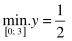
\includegraphics[width=0.75in,height=0.43403in]{./media/image8.png}
\end{center}
\textbf{C.}
\begin{center}
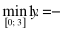
\includegraphics[width=0.80903in,height=0.33056in]{./media/image9.png}
\end{center}
\textbf{D.}
\begin{center}

\includegraphics[width=0.69097in,height=0.33056in]{./media/image10.png}
\end{center}
\end{quote}

\begin{enumerate}
\def\labelenumi{\arabic{enumi}.}
\setcounter{enumi}{9}
\item
  Sự phân huỷ của rác thải hữu cơ có trong nước sẽ làm tiêu hao oxygen
  hoà tan trong nước. Nồng độ oxygen (mg/l) trong một hồ nước sau \(t\)
  giờ \emph{(}\(t \geq 0\)\emph{)} khi một lượng rác thải hữu cơ bị xả
  vào hồ được xấp xỉ bởi hàm số có đồ thị là đường cong
  \(y(t) = 5 - \frac{15t}{9t^{2} + 1}\). Nồng độ oxygen trong nước thấp
  nhất vào các thời điểm nào ?
\end{enumerate}

\textbf{A.} \(t = 0\). \textbf{B.} \(t = \frac{1}{4}\). \textbf{C.}
\(t = \frac{1}{3}\). \textbf{D.} \(t = 0,3\).

\begin{enumerate}
\def\labelenumi{\arabic{enumi}.}
\setcounter{enumi}{10}
\item
  Trong số các hình chữ nhật có cùng chu vi 16 cm, hình chữ nhật có diện
  tích lớn nhất bằng:
\end{enumerate}

\begin{quote}
\textbf{A.} 64 cm\textsuperscript{2}. \textbf{B.} 4
cm\textsuperscript{2}. \textbf{C.} 16 cm\textsuperscript{2}. \textbf{D.}
8 cm\textsuperscript{2}..
\end{quote}

\begin{enumerate}
\def\labelenumi{\arabic{enumi}.}
\setcounter{enumi}{11}
\item
  Cho tứ diện\(ABCD\). Gọi \(M,\ N\) lần lượt là trung điểm của
  \(AB,\ CD\) và \(G\) là trung điểm của \emph{MN}. Trong các khẳng định
  sau, khẳng định nào \textbf{sai?}
\end{enumerate}

\begin{quote}
\textbf{A.}
\(\overrightarrow{MA} + \overrightarrow{MB} + \overrightarrow{MC} + \overrightarrow{MD} = 4\overrightarrow{MG}\)
\textbf{B.}
\(\overrightarrow{GA} + \overrightarrow{GB} + \overrightarrow{GC} = \overrightarrow{GD}\)

\textbf{C.}
\(\overrightarrow{GA} + \overrightarrow{GB} + \overrightarrow{GC} + \overrightarrow{GD} = \overrightarrow{0}\)
\textbf{D.}
\(\overrightarrow{GM} + \overrightarrow{GN} = \overrightarrow{0}\).
\end{quote}

\textbf{PHẦN II. Câu trắc nghiệm đúng sai.} Thí sinh trả lời từ câu 13
đến câu 16. Trong mỗi ý \textbf{a), b), c), d)} ở mỗi câu, thí sinh chọn
đúng (Đ) hoặc sai (S).

\begin{enumerate}
\def\labelenumi{\arabic{enumi}.}
\setcounter{enumi}{12}
\item
  Cho hình lăng trụ tam giác đều \(ABC.A^{'}B^{'}C^{'}\) có tất cả các
  cạnh bằng \(a\). \(G\)là trọng tâm tam giác \(ABC\).
\end{enumerate}

\begin{quote}
\textbf{a)} \(\overrightarrow{AB} = \overrightarrow{AC}\).

\textbf{b)}
\(\overrightarrow{CC^{'}} + \overrightarrow{AB} = \overrightarrow{AB^{'}}\).

\textbf{c)}
\(\overrightarrow{A^{'}G} = \overrightarrow{A^{'}A} + \overrightarrow{A^{'}B} + \overrightarrow{A^{'}C}\).

\textbf{d)}
\(\left| \overrightarrow{A^{'}A} + \overrightarrow{A^{'}B} + \overrightarrow{A^{'}C} \right| = \frac{2a\sqrt{3}}{3}\).
\end{quote}

\begin{enumerate}
\def\labelenumi{\arabic{enumi}.}
\setcounter{enumi}{13}
\item
  Cho hàm số \(f(x) = \frac{x^{2} - 2x - 3}{x + 2}\) có đồ thị \((C)\).
  Các mệnh đề sau đây đúng hay sai?
\end{enumerate}

\begin{quote}
\textbf{a)} Đồ thị hàm số có đường tiệm cận đứng là \(x = - 2\);

\textbf{b)} Đồ thị hàm số có đường tiệm cận xiên là \(y = x + 1\);

\textbf{c)} Tọa độ giao điểm của hai đường tiệm cận của đồ thị hàm số là
\(I( - 2; - 6)\);

\textbf{d)} Đường tiệm cận xiên của đồ thị hàm số cắt hai trục tọa độ
lần lượt tại hai điểm \(A,B\)tạo với hai trục tọa độ một tam giác có
diện tích bằng 16.
\end{quote}

\begin{enumerate}
\def\labelenumi{\arabic{enumi}.}
\setcounter{enumi}{14}
\item
  Cho hàm số \(y = f(x)\) có bảng xét dấu đạo hàm như sau:
\end{enumerate}

\begin{quote}
\begin{center}
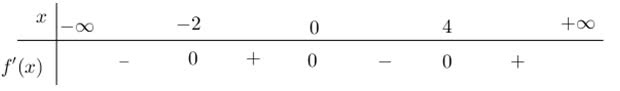
\includegraphics[width=4.45in,height=0.65278in]{./media/image11.jpg}
\end{center}

\textbf{a)} Hàm số nghịch biến trên khoảng \((0; + \infty)\).

\textbf{b)} Hàm số có \(3\) điểm cực trị.

\textbf{c)} Hàm số\(y = f(1 - x)\) nghịch biến trên khoảng \((0;2)\).

\textbf{d)} Hàm số \(g(x) = f(1 - x) + \frac{x^{3}}{3} - 2x^{2} + 3x\)
đạt cực tiểu tại điểm \(x = 3\).
\end{quote}

\begin{enumerate}
\def\labelenumi{\arabic{enumi}.}
\setcounter{enumi}{15}
\item
  Độ cao (mét) của một viên đạn được bắn lên trời từ một vị trí cách mặt
  đất 20m theo phương thẳng đứng với vận tốc ban đầu \(294m/s\) (bỏ qua
  sức cản của không khí) là \(h(t) = 20 + 294t - 4,9t^{2}\). Các mệnh đề
  sau đúng hay sai?
\end{enumerate}

\begin{quote}
\textbf{a)} Vận tốc ban đầu của viên đạn là \(294m/s\).

\textbf{b)} Vận tốc của viên đạn sau \(2\) giây là \(292m/s\).

\textbf{c)} Viên đạn đạt độ cao lớn nhất tại thời điểm \(t = 25\)giây.

\textbf{d)} Viên đạn đạt độ cao lớn nhất là \(4430(m)\).
\end{quote}

\textbf{PHẦN III. Câu trắc nghiệm trả lời ngắn.} Thí sinh trả lời từ câu
17 đến câu 22.

\begin{enumerate}
\def\labelenumi{\arabic{enumi}.}
\setcounter{enumi}{16}
\item
  Ta đã biết trọng tâm của tứ diện \(ABCD\) là một điểm \(I\) thoả mãn
  \(\overrightarrow{AI} = 3\overrightarrow{IG}\), ở đó \(G\) là trọng
  tâm của \(\Delta BCD\). Áp dụng tính chất trên để tính khoảng cách từ
  trọng tâm của một khối rubik (đồng chất) hình tứ diện đều đến một mặt
  của nó, biết rằng chiều cao của khối rubik là \(8\ cm\).
\end{enumerate}

\begin{quote}
\begin{center}
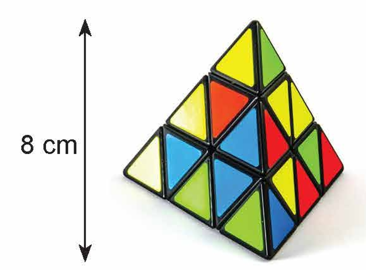
\includegraphics[width=1.66545in,height=1.22861in]{./media/image12.png}
\end{center}
\end{quote}

\begin{enumerate}
\def\labelenumi{\arabic{enumi}.}
\setcounter{enumi}{17}
\item
  Cho hàm số \(y = f(x)\) có bảng biến thiên như sau:
\end{enumerate}

\begin{center}
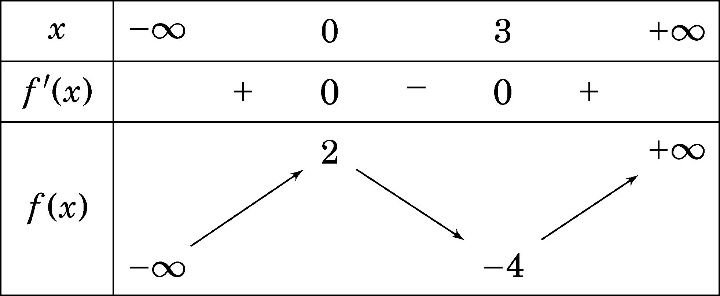
\includegraphics[width=3.27153in,height=1.34653in]{./media/image13.jpeg}
\end{center}

Giá trị cực tiểu của hàm số đã cho bằng bao nhiêu?

\begin{enumerate}
\def\labelenumi{\arabic{enumi}.}
\setcounter{enumi}{18}
\item
  Cho hai vị trí \(A\), \(B\) cách nhau \(615m\), cùng nằm về một phía
  bờ sông như hình vẽ. Khoảng cách từ \(A\) và từ \(B\) đến bờ sông lần
  lượt là \(118m\) và \(487m\). Một người đi từ \(A\) đến bờ sông để lấy
  nước mang về \(B\)\emph{.} Đoạn đường ngắn nhất mà người đó có thể đi
  là (làm tròn đến hàng đơn vị):
\item
  Khoảng cách giữa hai điểm cực trị của đồ thị hàm số
  \(y = x^{3} - 3x + 1\) là (kết quả làm tròn đến hàng phần trăm)
\item
  Cho hàm số \(y = \frac{x - 2}{x + 1}\). Kí hiệu
  \(M = \underset{\lbrack 2;3\rbrack}{Maxy}\) và
  \(m = \underset{\lbrack 2;3\rbrack}{Miny}\). Khi đó \(M + m\) bằng
\item
  Trong không gian, xét hệ trục tọa độ \(Oxyz\), có gốc \(O\) trùng với
  vị trí của một giàn khoan trên biển, mặt phẳng \((Oxy)\) trùng với mặt
  biển (được coi là mặt phẳng), với \(Ox\) hướng về phía tây,
  \(Oy\)hướng về phía nam, \(Oz\) hướng lên trời. Đơn vị đo trong
  \(Oxyz\) tính theo \(\text{km}\). Radar đặt tại giàn khoan phát hiện
  một tàu thám hiểm có vị trí cách giàn khoan \(10km\) về phía tây,
  \(5km\)về phía nam, và ở độ sâu cách mặt nước biển 4359\emph{m}.
  Khoảng cách từ radar tới tàu thám hiểm tính theo đơn vị \emph{km} làm
  tròn đến hàng đơn vị là
\end{enumerate}

\begin{center}
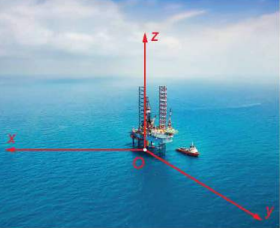
\includegraphics[width=2.91707in,height=2.37533in]{./media/image14.png}
\end{center}


\end{document}
